

\setlength{\abovedisplayskip}{3pt}
\setlength{\belowdisplayskip}{3pt}
\setlength{\abovedisplayshortskip}{3pt}
\setlength{\belowdisplayshortskip}{3pt}

	\thispagestyle{empty}
	\rule{\linewidth}{1pt}
	
	\vspace{6pt}				%Die Leerzeilen müssen tatsächlich da sein, sonst funktioniert das nicht
	
	\begin{minipage}{0.6\textwidth}
		\begin{flushleft} 
		\Autor\\
		\Profs
		\end{flushleft}
	\end{minipage}
	\begin{minipage}{0.39\textwidth}
		\begin{flushright}
			Universität Hamburg
		\end{flushright}
	\end{minipage}

	\rule{\linewidth}{1pt}\\
	\begin{center}
		\Large{\textsf{\titel}}\\
		\small\textsf{Version vom \today}
\vspace{8pt}
\end{center}


\begin{figure}[htbp]
    \centering
    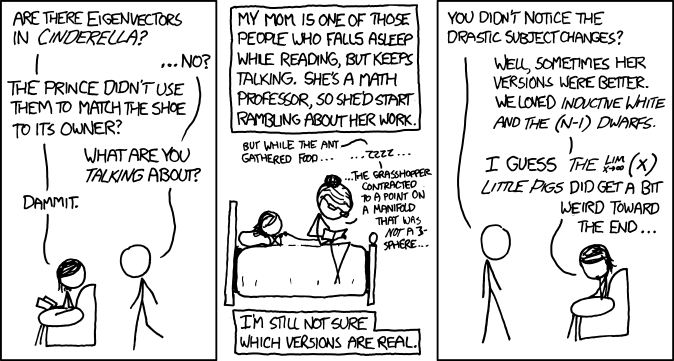
\includegraphics[width=.55\textwidth]{Dateien/00xkcd.png}\\
    Erzählt uns, wenn es euch auch so geht. Wir kennen da einen guten Arzt.\\
    Bildquelle: \url{https://xkcd.com/872/}
\end{figure}
\vfill
Moin, dies sind die informellen Notizen begleitend zu unserem MfP2-Tutorium.\\
Diese sind primär als unsere eigene Vorbereitung auf die Tutorien zu sehen, ihr könnt sie aber gerne nutzen, um euer Wissen zur Vorlesung zu vertiefen.\\
Hier greifen wir einige der wichtigsten Sätze und Definitionen auf, um diese dann durch Beispiele zu veranschaulichen. Lasst euch nicht davon abschrecken, dass wir manchmal noch ein bisschen mehr dazu schreiben - Wir empfehlen sogar eher, dies als Nachschlagewerk zu nutzen, das \Skript{} ersetzt es auf keinen Fall!\\
Wichtig ist auch: Viele Satzbezeichnungen und die Nummerierung der Definitionen, Sätze und Beispiele sind nur \red{inoffiziell} und dienen der internen Übersicht in diesen Notizen, ihr solltet also bei der Bearbeitung eurer Übungsaufgaben nicht darauf verweisen (nehmt stattdessen lieber die Folien im Skript).\\
Viele weitere Aufgaben zur Klausurvorbereitung findet ihr in unserer Aufgabensammlung.\\
Bei Anmerkungen oder Fragen (es haben sich bestimmt noch einige Fehler eingeschlichen) schreibt uns einfach bei Telegram oder schickt uns eine E-Mail an fabian.balzer@studium.uni-hamburg.de.\\\\
Viel Erfolg beim Lernen und Üben!\\
:)
\cfoot{\pagemark}
